\subsection{Removing cards from a partition}
\begin{figure}[htp]
\begin{center}
  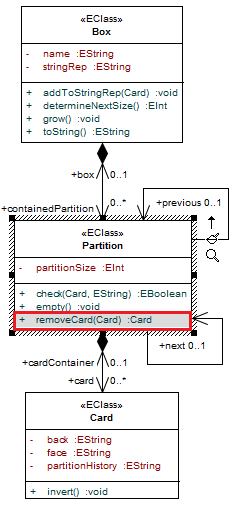
\includegraphics[width=0.7\textwidth]{pics/sdmBilder/removeCard/sdm01RAW}
  \caption{Double-click a method to implement it.}  
  \label{fig:sdm_start}
\end{center}
\end{figure}

\begin{figure}[htp]
\begin{center}
  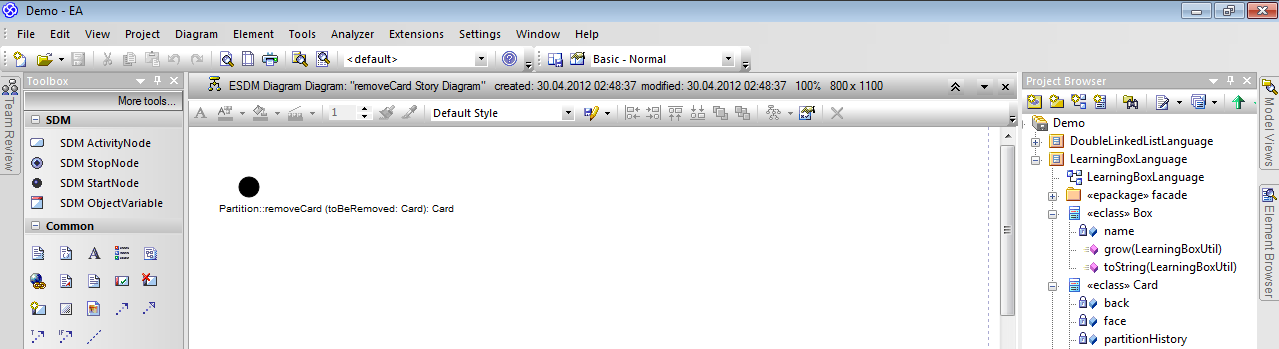
\includegraphics[width=0.7\textwidth]{pics/sdmBilder/removeCard/sdm02RAW}
  \caption{Generated SDM diagram and start node.}  
  \label{fig:sdm_skeleton}
\end{center}
\end{figure}

\begin{figure}[htp]
\begin{center}
  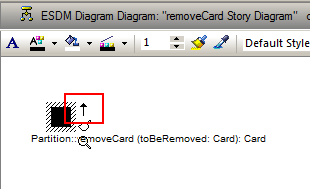
\includegraphics[width=0.7\textwidth]{pics/sdmBilder/removeCard/sdm03RAW}
  \caption{Quick link in SDM diagram to create new activity node.}  
  \label{fig:sdm_quicklink}
\end{center}
\end{figure}

\begin{figure}[htp]
\begin{center}
  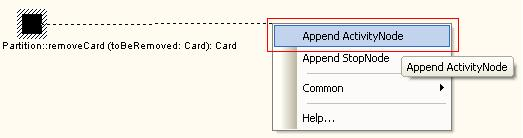
\includegraphics[width=0.7\textwidth]{pics/sdmBilder/removeCard/sdm04RAW}
  \caption{Create new activity node.}  
  \label{fig:sdm_new_activity_node}
\end{center}
\end{figure}

\begin{figure}[htp]
\begin{center}
  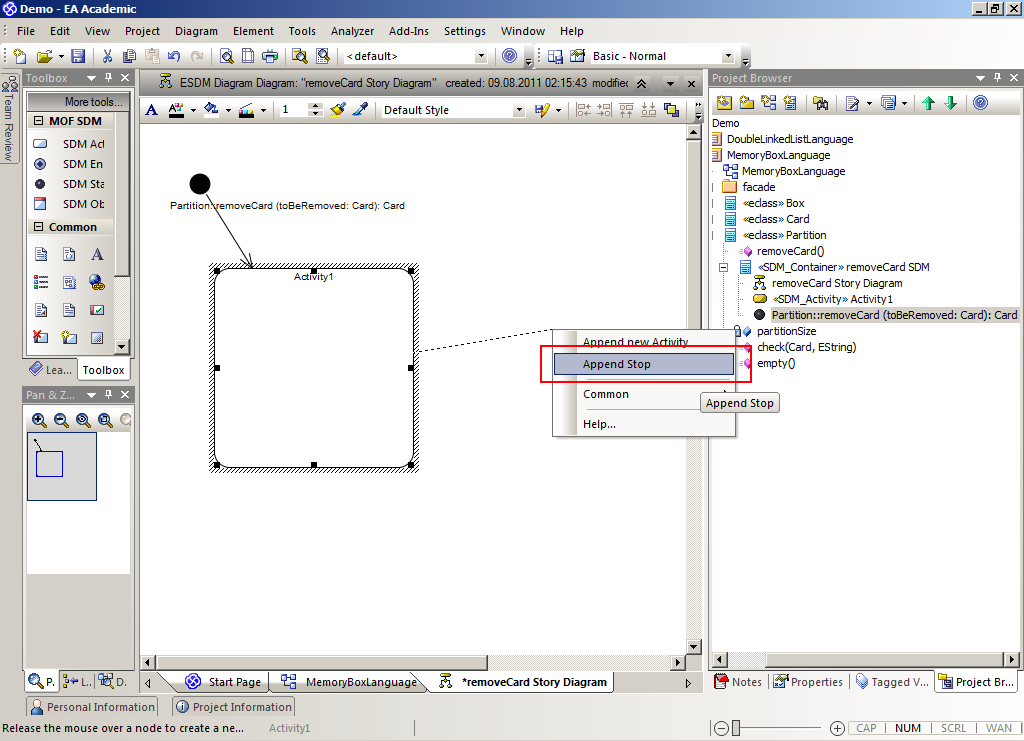
\includegraphics[width=0.7\textwidth]{pics/sdmBilder/removeCard/sdm05RAW}
  \caption{Complete activity with a stop node.}  
  \label{fig:sdm_stop_node}
\end{center}
\end{figure}

\begin{figure}[htp]
\begin{center}
  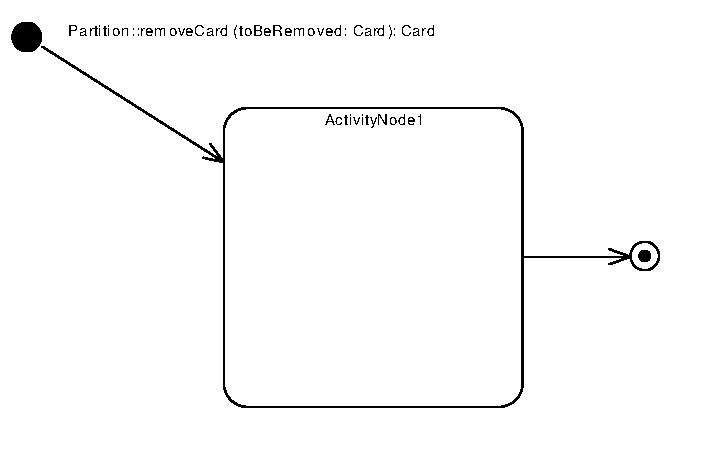
\includegraphics[width=0.7\textwidth]{pics/sdmBilder/removeCard/sdm06RAW}
  \caption{Control flow modelled as a simple activity diagram.}  
  \label{fig:sdm_complete_control_flow}
\end{center}
\end{figure}

\begin{figure}[htp]
\begin{center}
  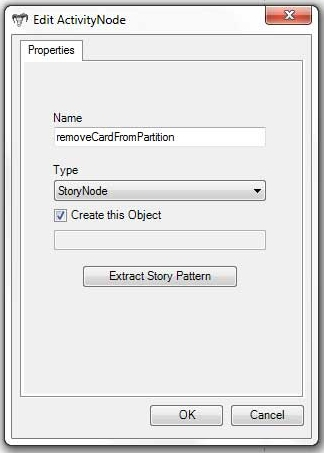
\includegraphics[width=0.7\textwidth]{pics/sdmBilder/removeCard/sdm07RAW}
  \caption{Start modelling story pattern in activity node.}  
  \label{fig:story_pattern}
\end{center}
\end{figure}

\begin{figure}[htp]
\begin{center}
  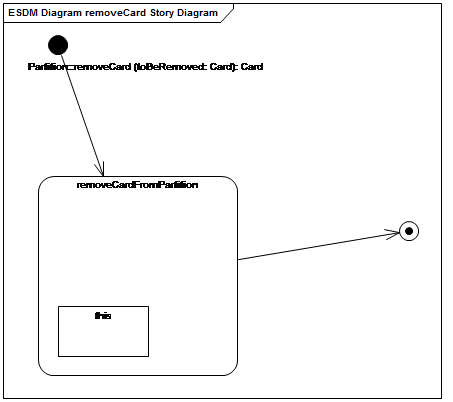
\includegraphics[width=0.7\textwidth]{pics/sdmBilder/removeCard/sdm08RAW}
  \caption{Story pattern with just one object variable for \texttt{this}.}  
  \label{fig:sdm_complete_control_flow}
\end{center}
\end{figure}

\begin{figure}[htp]
\begin{center}
  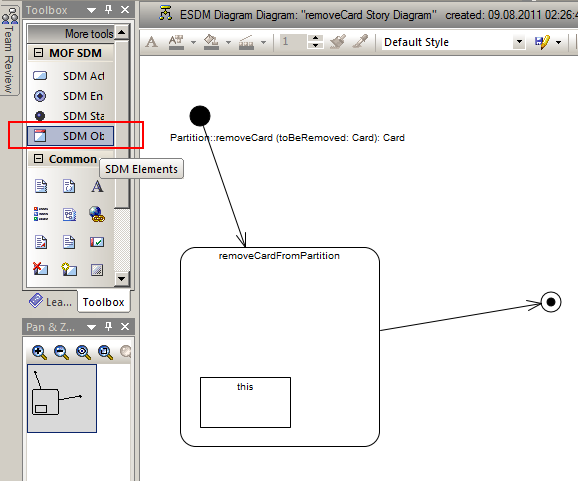
\includegraphics[width=0.7\textwidth]{pics/sdmBilder/removeCard/sdm09RAW}
  \caption{Add a new object variable from the tool-box.}  
  \label{fig:tool_box}
\end{center}
\end{figure}

\begin{figure}[htp]
\begin{center}
  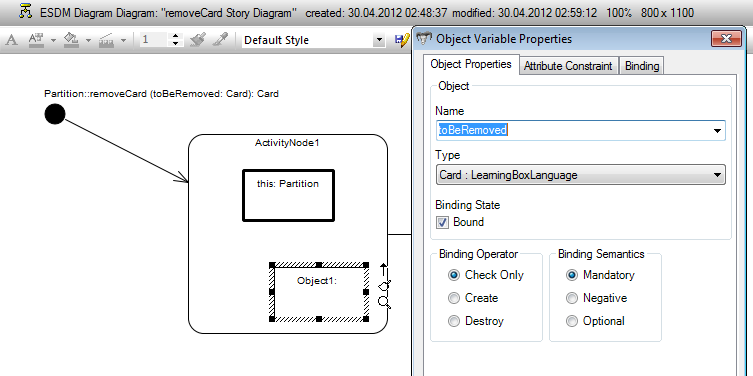
\includegraphics[width=0.7\textwidth]{pics/sdmBilder/removeCard/sdm10RAW}
  \caption{Specify properties of the added object variable.}  
  \label{fig:object_variable_properties}
\end{center}
\end{figure}

\begin{figure}[htp]
\begin{center}
  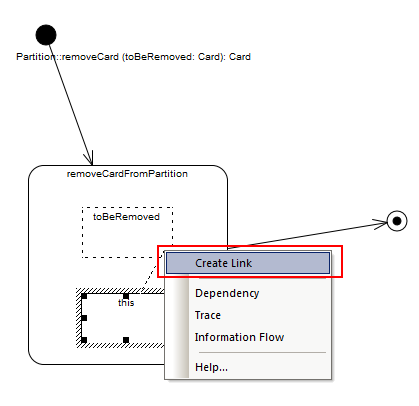
\includegraphics[width=0.7\textwidth]{pics/sdmBilder/removeCard/sdm11RAW}
  \caption{Create a link variable.}  
  \label{fig:link_variable}
\end{center}
\end{figure}

\begin{figure}[htp]
\begin{center}
  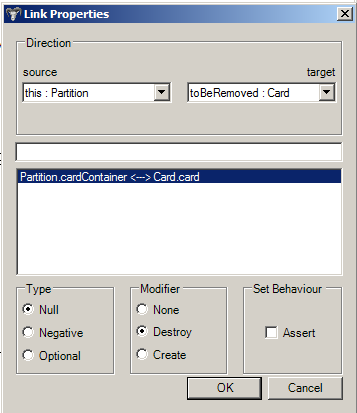
\includegraphics[width=0.7\textwidth]{pics/sdmBilder/removeCard/sdm12RAW}
  \caption{Specify properties for created link variable.}  
  \label{fig:link_variable_properties}
\end{center}
\end{figure}

\begin{figure}[htp]
\begin{center}
  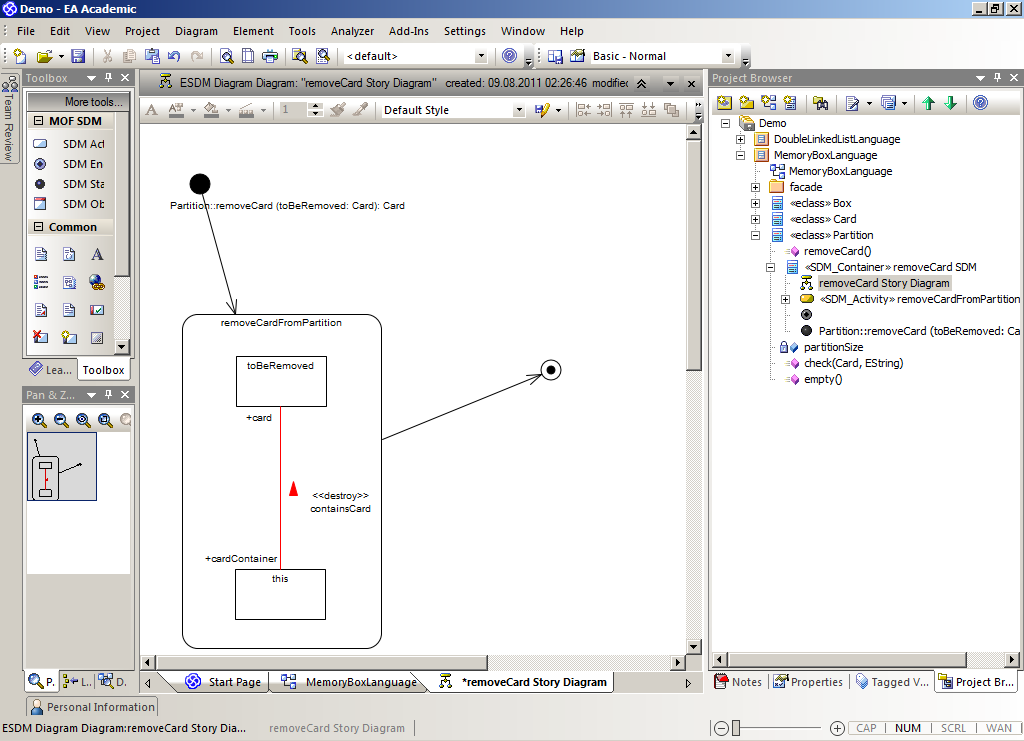
\includegraphics[width=0.7\textwidth]{pics/sdmBilder/removeCard/sdm13RAW}
  \caption{Status after creating link variable}  
  \label{fig:link_variable_added}
\end{center}
\end{figure}

\begin{figure}[htp]
\begin{center}
  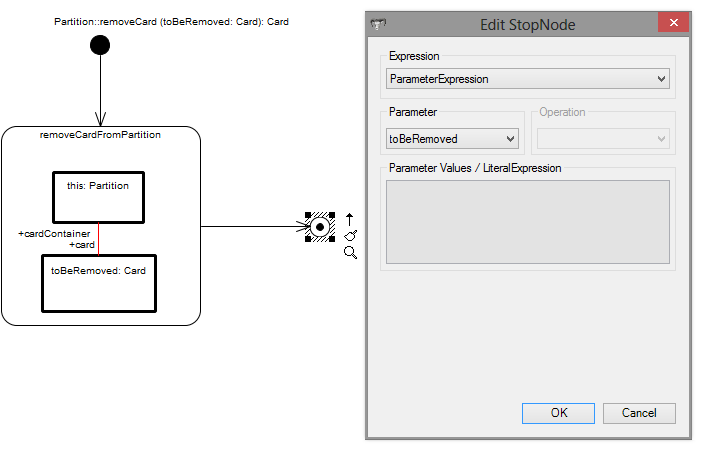
\includegraphics[width=0.7\textwidth]{pics/sdmBilder/removeCard/sdm14RAW}
  \caption{Adding a return value to the stop node.}  
  \label{fig:stop_node_return_value}
\end{center}
\end{figure}

\begin{figure}[htp]
\begin{center}
  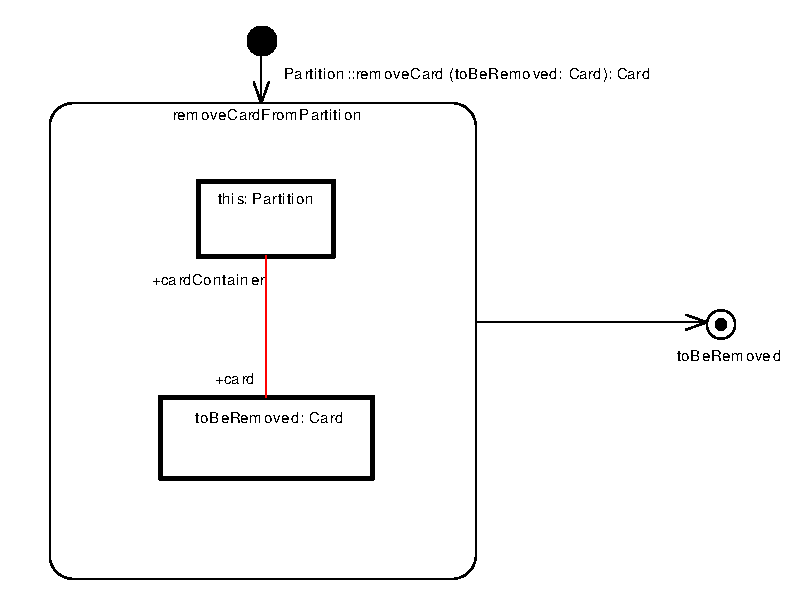
\includegraphics[width=0.7\textwidth]{pics/sdmBilder/removeCard/sdm15}
  \caption{Complete SDM for \texttt{Partition::removeCard)}.}  
  \label{fig:sdm_complete_control_flow}
\end{center}
\end{figure}

\clearpage